%----------------------------------------------------------------------------------------
%    PACKAGES AND THEMES
%----------------------------------------------------------------------------------------

\documentclass[aspectratio=169,xcolor=dvipsnames]{beamer}
\usetheme{SimplePlus}
\usepackage[polish]{babel}
\usepackage[T1]{fontenc}
\usepackage{graphicx} % Allows including images

%----------------------------------------------------------------------------------------
%    TITLE PAGE
%----------------------------------------------------------------------------------------

\title{Tworzenie podsumowań tekstu}
\subtitle{Przetwarzanie języka naturalnego}

\author{Piotr Zalewski Kacper Świderek}


%----------------------------------------------------------------------------------------
%    PRESENTATION SLIDES
%----------------------------------------------------------------------------------------

\begin{document}

\begin{frame}
    \titlepage
\end{frame}

%------------------------------------------------
\section{Cel Projektu}
%------------------------------------------------

\begin{frame}{Cel Projektu}
    Opracowanie systemu, który automatycznie generuje zwięzłe i informacyjne
podsumowania dla tekstów wejściowych pozwalając użytkownikowi na szybkie
zapoznanie się z kluczowymi informacjami zawartymi w obszernych dokumentach,
bez konieczności ich pełnego czytania.
\end{frame}

%------------------------------------------------

\begin{frame}{Motywacja i wyzwania}
    W dzisiejszym świecie natłok informacji utrudnia ludziom szybkie przyswajanie
kluczowych treści. Odczytanie pełnych artykułów czy dokumentów może być
czasochłonne, a brak podsumowań znacząco ogranicza możliwości szybkiego
podejmowania decyzji.\\~

Wyzwaniem było stworzenie podsumowania całego teksu metodą abstrakcyjną oraz
 ograniczenie jego długości.
\end{frame}

%------------------------------------------------

\begin{frame}{Teoretyczne podstawy rozwiązania}
    \begin{columns}[c] % The "c" option specifies centered vertical alignment while the "t" option is used for top vertical alignment

        \column{.45\textwidth} % Left column and width
        \textbf{Ekstrakcyjne}
        \begin{itemize}
            \item TF-IDF
            \item TextRank \\~
        \end{itemize}

        \textbf{Ocena jakości podsumowań}
        \begin{itemize}
            \item ROUGEscore
            \item BARTscore
        \end{itemize}

        \column{.45\textwidth} % Right column and width
        \textbf{Abstrakcyjne}
        \begin{itemize}
            \item T5
            \item BART
            \item Pegasus
        \end{itemize}
    \end{columns}
\end{frame}

%------------------------------------------------

\begin{frame}{Opis metodyki}
    Omówienie kroków realizacji zadania:
    \begin{itemize}
        \item Przetwarzanie tekstu
        \item wygenerowanie podsumowania
        \item Ewaluacja
    \end{itemize}
\end{frame}

%------------------------------------------------

\begin{frame}{Wykorzystane narzędzia i biblioteki}
    \begin{itemize}
        \item \textbf{spacy}: segmentacja tekstu
        \item \textbf{TextRank}: generowanie podsumowań ekstrakcyjnych
        \item \textbf{sklearn}: TF-IDF
        \item \textbf{transformers}: abstrakcyjne podsumowania, BART, Pegasus, T5
        \item \textbf{rouge\_score}: ewaluacja podsumowania
        \item \textbf{bert\_score}: ewaluacja podsumowania
    \end{itemize}
\end{frame}

%------------------------------------------------

\begin{frame}{Przykłady użycia programu}
    \begin{figure}
        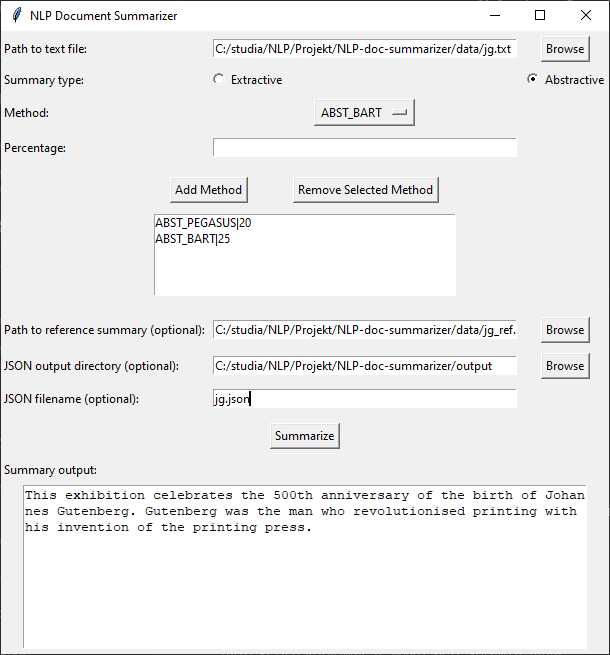
\includegraphics[width=0.6\linewidth]{gui_example.PNG}
        \end{figure}
\end{frame}

%------------------------------------------------

\begin{frame}{Wyniki testów i ewaluacja}
    \begin{figure}
    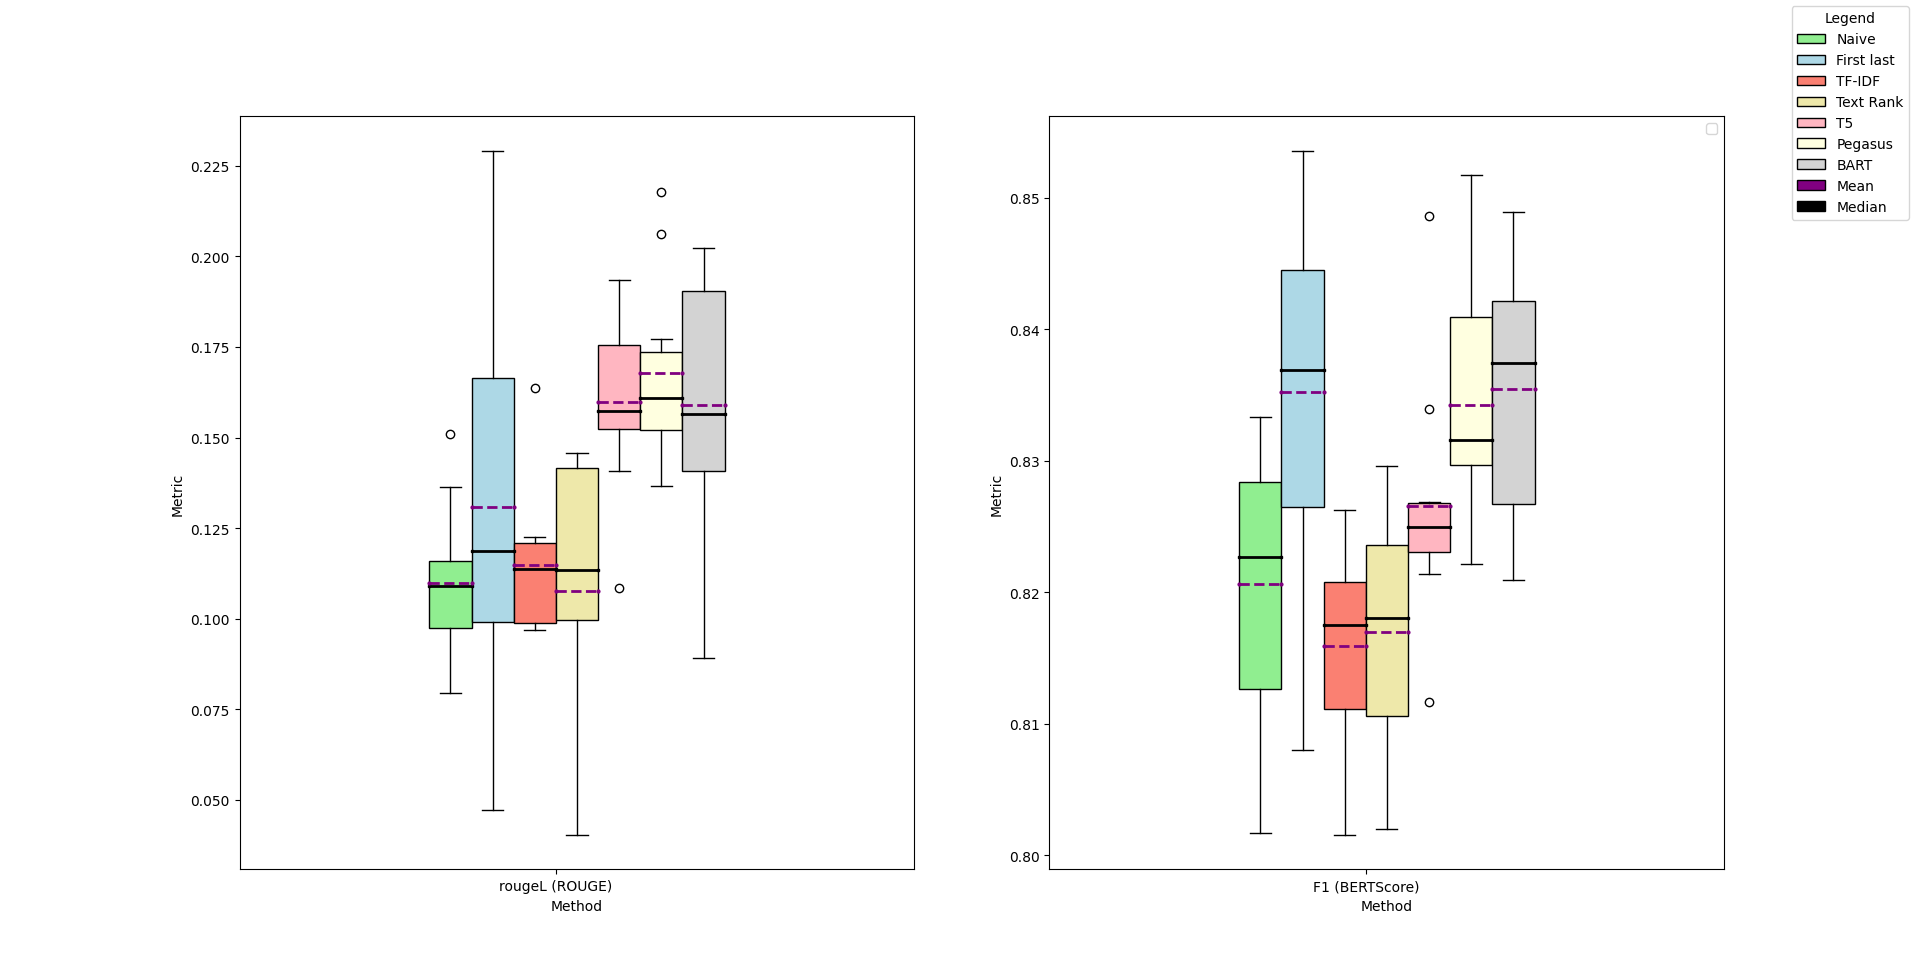
\includegraphics[width=0.8\linewidth]{war_and_peace.png}
    \caption{Wykresy pudełkowe, z wyników na danych rozdziałach książki
    \textit{War and peace}.}
    \end{figure}
\end{frame}

%------------------------------------------------

\begin{frame}{Problemy i rozwiązania}
    \begin{itemize}
        \item Problemy z jakością podsumowań abstrakcyjnych: powtarzające się słowa/frazy/zdania.
    \end{itemize}
\end{frame}

%------------------------------------------------

\begin{frame}{Możliwości rozwoju i ulepszenia}
    Propozycje rozszerzeń i ulepszeń projektu:
    \begin{itemize}
        \item Poprawa jakości podsumowań abstrakcyjnych.
        \item Integracja z większą ilością metod oceny jakości podsumowań.
        \item Rozszerzenie funkcjonalności GUI.
    \end{itemize}
\end{frame}

%----------------------------------------------------------------------------------------

\begin{frame}{Podsumowanie i wnioski}
    Krótkie podsumowanie kluczowych osiągnięć:
    \begin{itemize}
        \item Podsumowania ekstrakcyjne mogą przynosić zadowalające rezultaty dla krótkich tekstów.
        \item Metody abstrakcyjne są ogólnie lepsze od metod ekstrakcyjnych.
        \item Metoda \textit{Pegasus} otrzymała najwyższe wyniki.
    \end{itemize}
\end{frame}

%------------------------------------------------

\begin{frame}
    \Huge{\centerline{\textbf{Dziękujemy za uwagę}}}
\end{frame}

%----------------------------------------------------------------------------------------

\end{document}